\documentclass{standalone}
\usepackage{tikz}

\tikzset{
  svgfrag/.style 2 args={
    execute at begin scope={\special{dvisvgm:raw <g class="fragment #2" data-fragment-index="#1">}},
    execute at end scope={\special{dvisvgm:raw </g>}},
    execute at begin node={\special{dvisvgm:raw <g class="fragment #2" data-fragment-index="#1">}},
    execute at end node={\special{dvisvgm:raw </g>}},
  }
}

\begin{document}
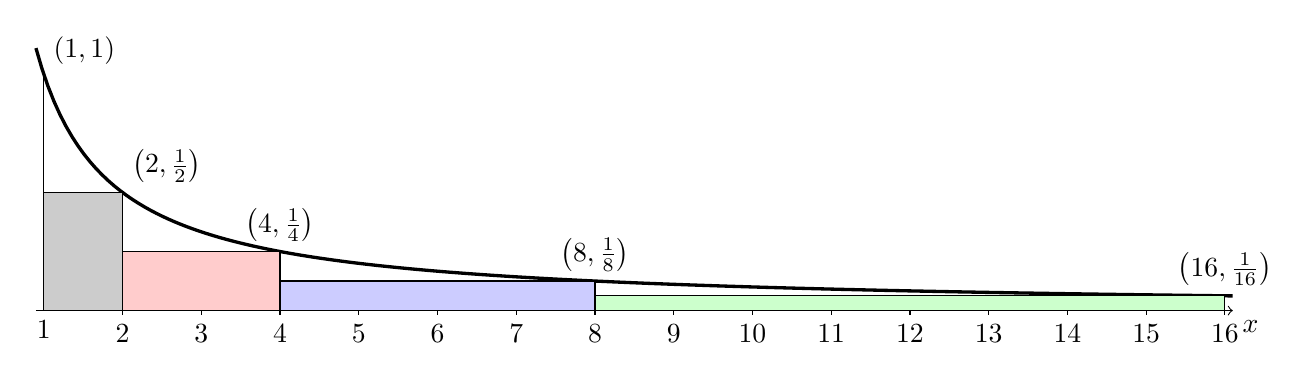
\begin{tikzpicture}[domain=0.9:16.1, yscale=3]
    \draw[->] (0.9,0) -- (16.1,0)node[below right]{$x$};
    \draw[very thick] plot[samples=200] (\x, {1/\x});
    \draw[thin] (1,1)node[above right]{$(1,1)$} -- (1,0)node[below]{$1$};
    \foreach \x in {2,...,16}{
        \draw (\x,0) +(0,.02) -- +(0,-.02)node[below]{$\x$};
    }
    \begin{scope}[svgfrag={1}{fade-in}]
        \draw[fill=black!20] (1,0) rectangle (2,0.5)node[above right]{$\left(2,\frac{1}{2}\right)$};
    \end{scope}
    \begin{scope}[svgfrag={2}{fade-in}]
        \draw[fill=red!20] (2,0) rectangle (4,0.25)node[above]{$\left(4,\frac{1}{4}\right)$};
    \end{scope}
    \begin{scope}[svgfrag={3}{fade-in}]
        \draw[fill=blue!20] (4,0) rectangle (8,0.125)node[above]{$\left(8,\frac{1}{8}\right)$};
    \end{scope}
    \begin{scope}[svgfrag={4}{fade-in}]
        \draw[fill=green!20] (8,0) rectangle (16,0.0625)node[above]{$\left(16,\frac{1}{16}\right)$};
    \end{scope}
\end{tikzpicture}
\end{document}
